
\subsection{Noise Robustness Comparisons}


Here we present results for noise robustness experiments. These tests were performed on data captured via the ASUS Xtion PRO LIVE camera. These data were presented in section \ref{TestDataSection} and example frames are shown in Appendix \ref{AppendixA}. Frames from these data-sets are transformed by various transformations with varying amounts of noise added. This noise is measured in both SNR and noise range. A noise range of 1.0 means random noise within the range [$-0.5$, $0.5$] was added. SNR is measured in decibels. Accuracy was measured using the percent of points matched to a close neighbour post registration. This metric was discussed in section \ref{TestDataSection}. 

\subsubsection{Rotation Registration}

\begin{figure}[!htb]
\centering
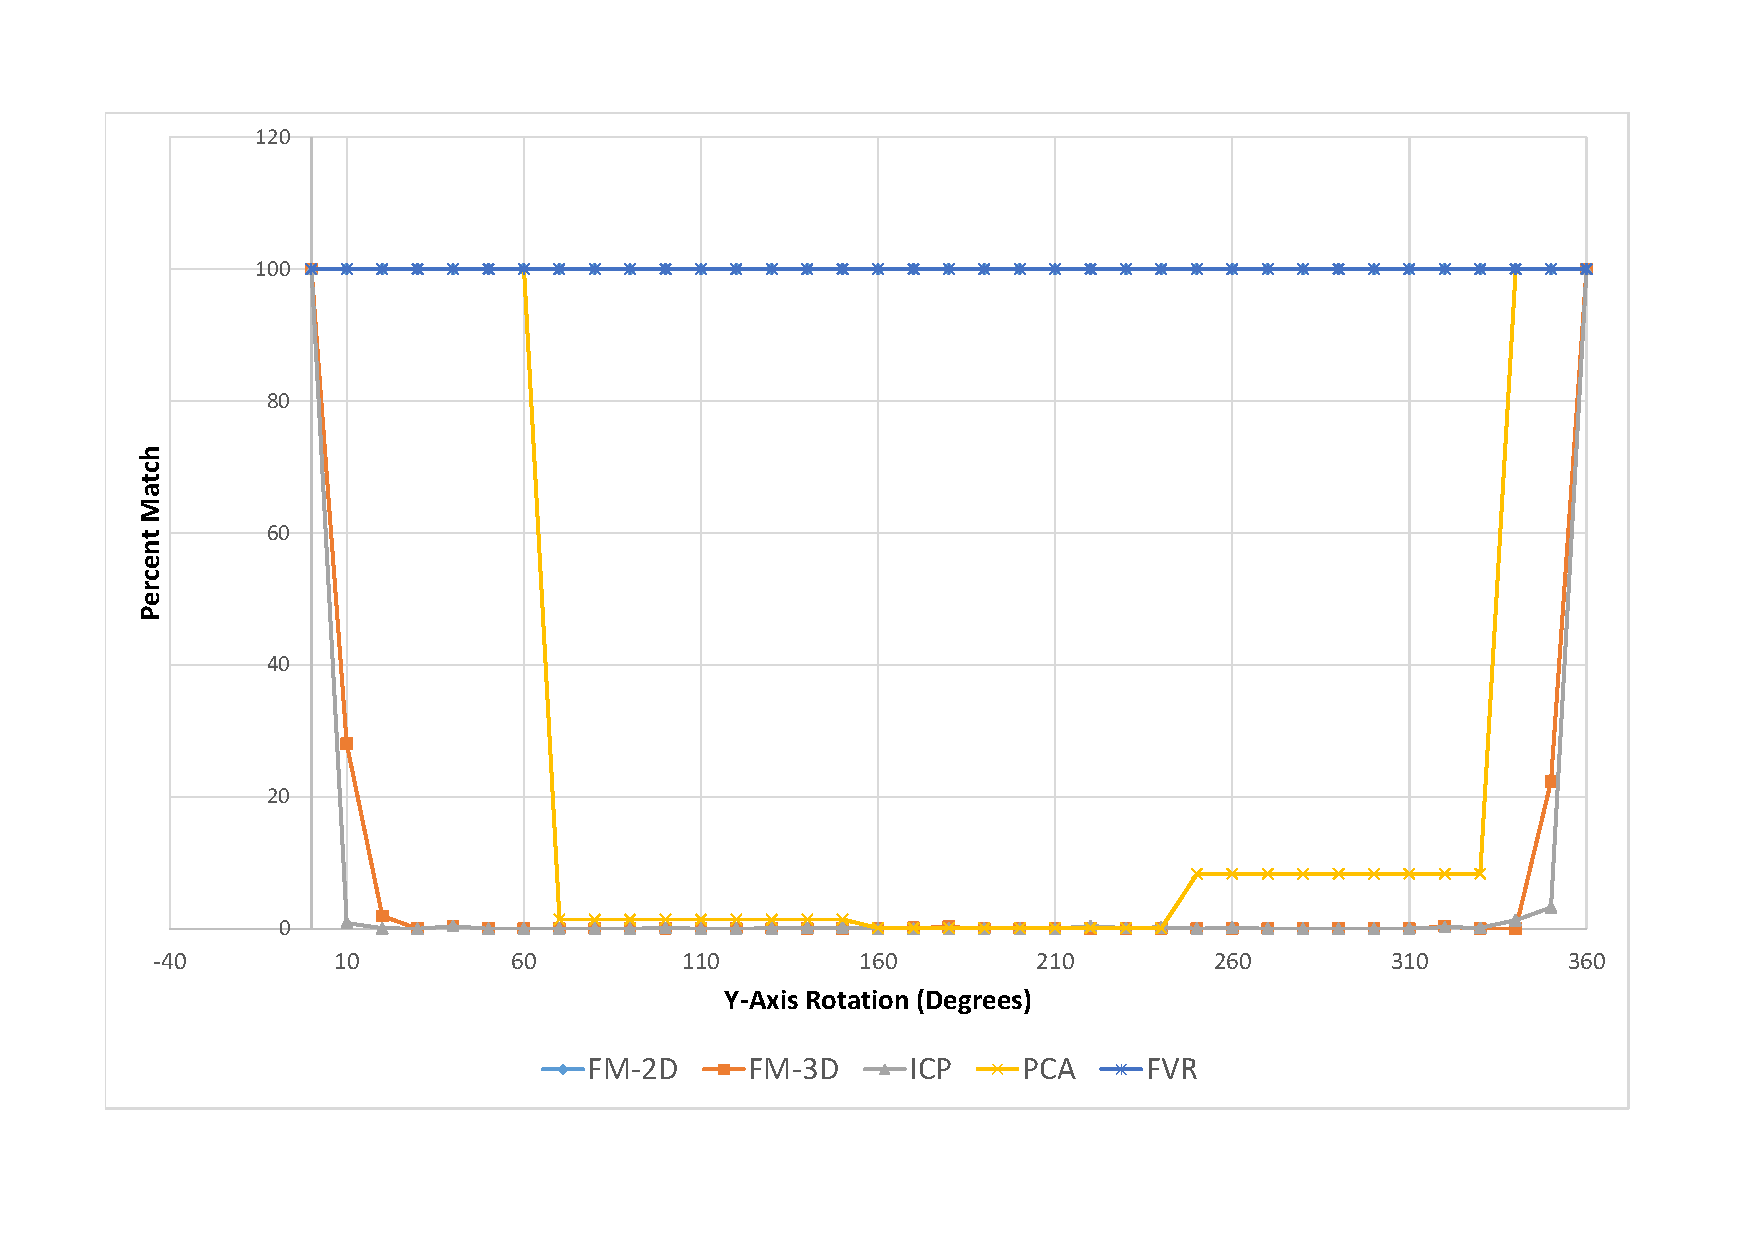
\includegraphics[width=4.0in]{images/results/noise/YRNoise0}
\caption{Percent Match for Y-Axis Registration with an Infinite SNR and noise range of $0$.}
\label{fig:YRNoise0}
\end{figure}

In the first set of experiments, scanned 3D data was rotated about the Y-axis. Figure \ref{fig:YRNoise0} shows results with an infinite SNR. The 2D-FM method and FVR achieved perfect results. PCA performed next best, but failed to register degrees above 70. Since no noise was present, PCA was truly accurate, however some axes were flipped. This may be fixed by testing the data for flipped axes. FM-3D and ICP fell away much earlier. ICP is not good at registering significant transforms and FM-3D also does not perform well as quantization errors are higher since its data was quantized into volumes of size $128^3$. \\

\begin{figure}[!htb]
\centering
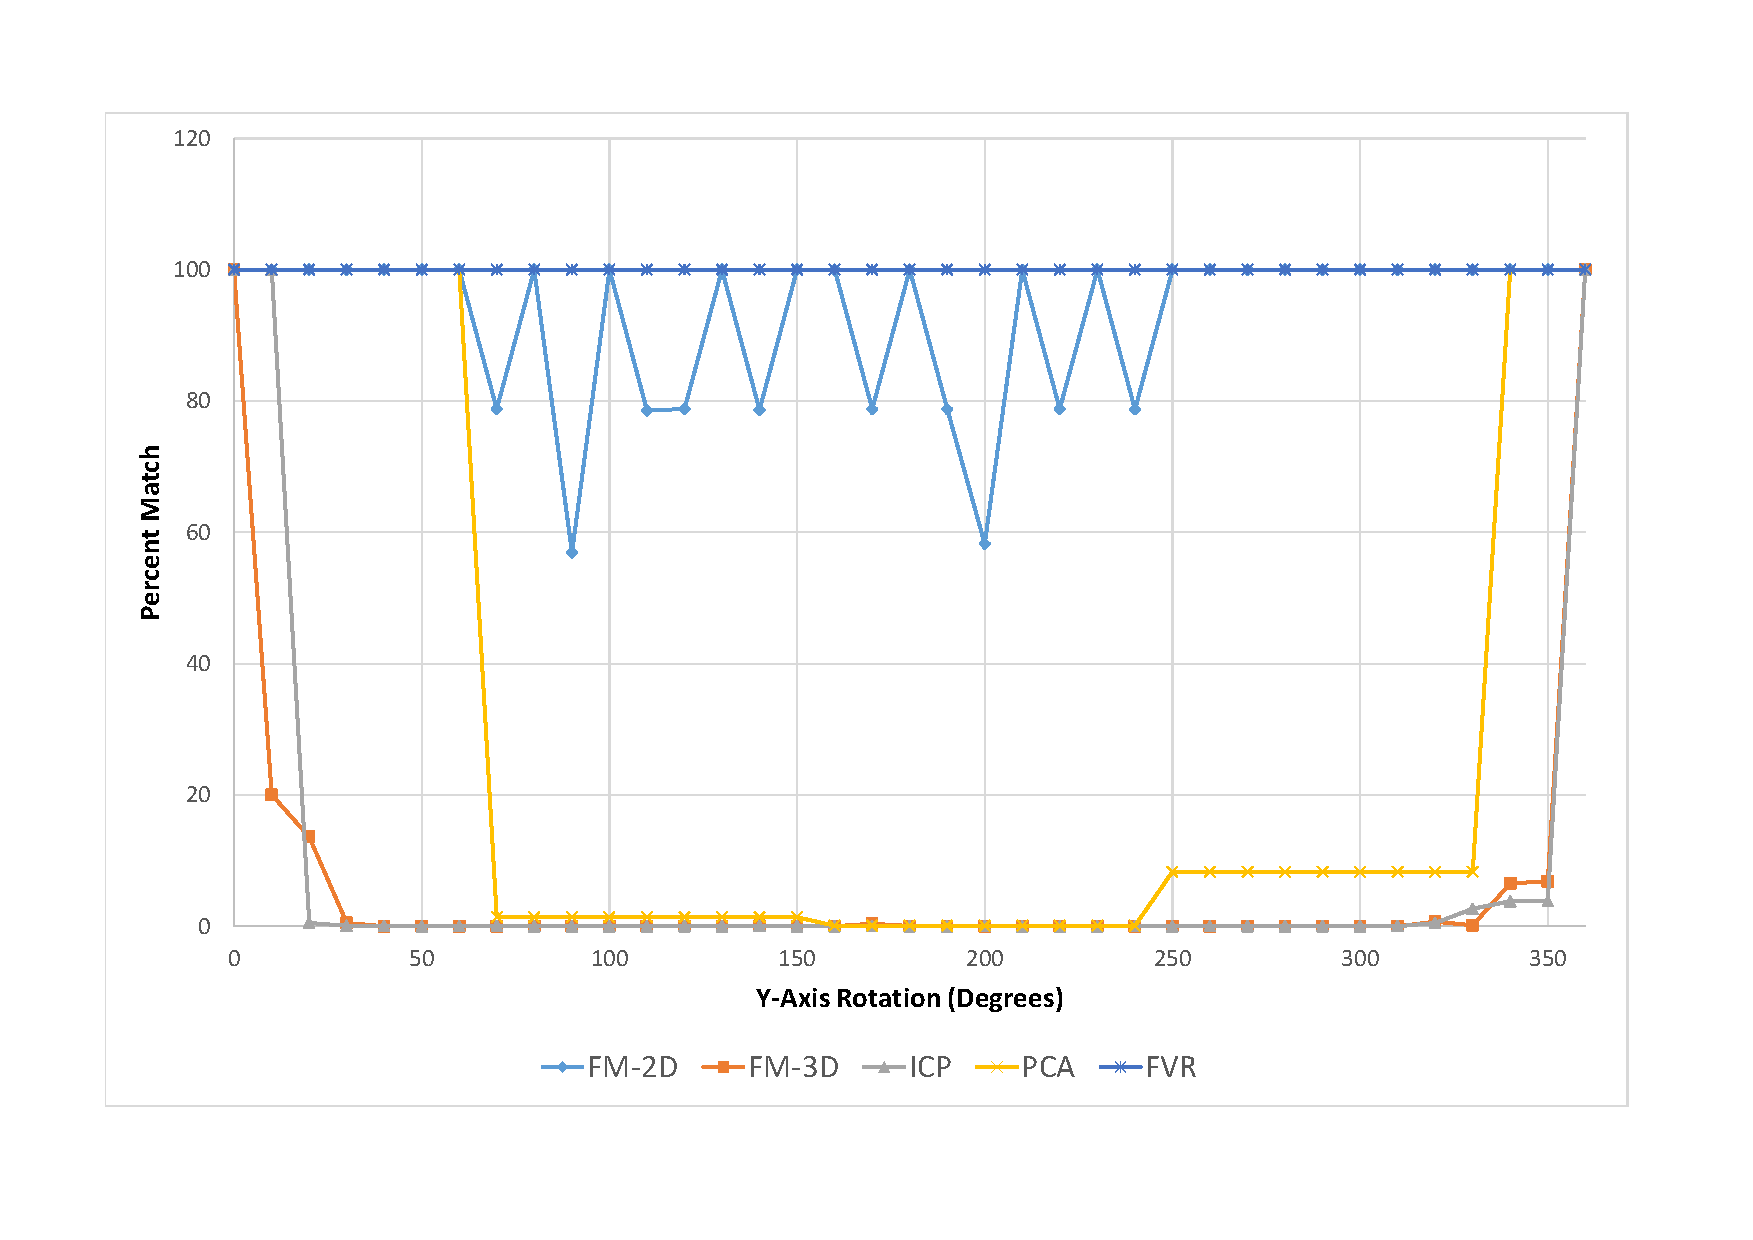
\includegraphics[width=4.0in]{images/results/noise/YRNoise1}
\caption{Percent Match for Y-Axis Registration with an SNR of and noise range of $10300$ and noise range of $1.0$.}
\label{fig:YRNoise1}
\end{figure}

For the results in figure \ref{fig:YRNoise1} the noise was dropped to a SNR of $10300$. Here, similar results are seen. For FM-2D however, registration error occurs during registration of larger rotations (rotations above 180 degrees are considered small in terms of absolute rotational shift). In figure \ref{fig:YRNoise2} we reduced the SNR to $2580$ which caused more error in FM-2D. These results suggest that for simple Y-axis rotation, FVR is superior in terms of noise robustness.  \\

\begin{figure}[!htb]
\centering
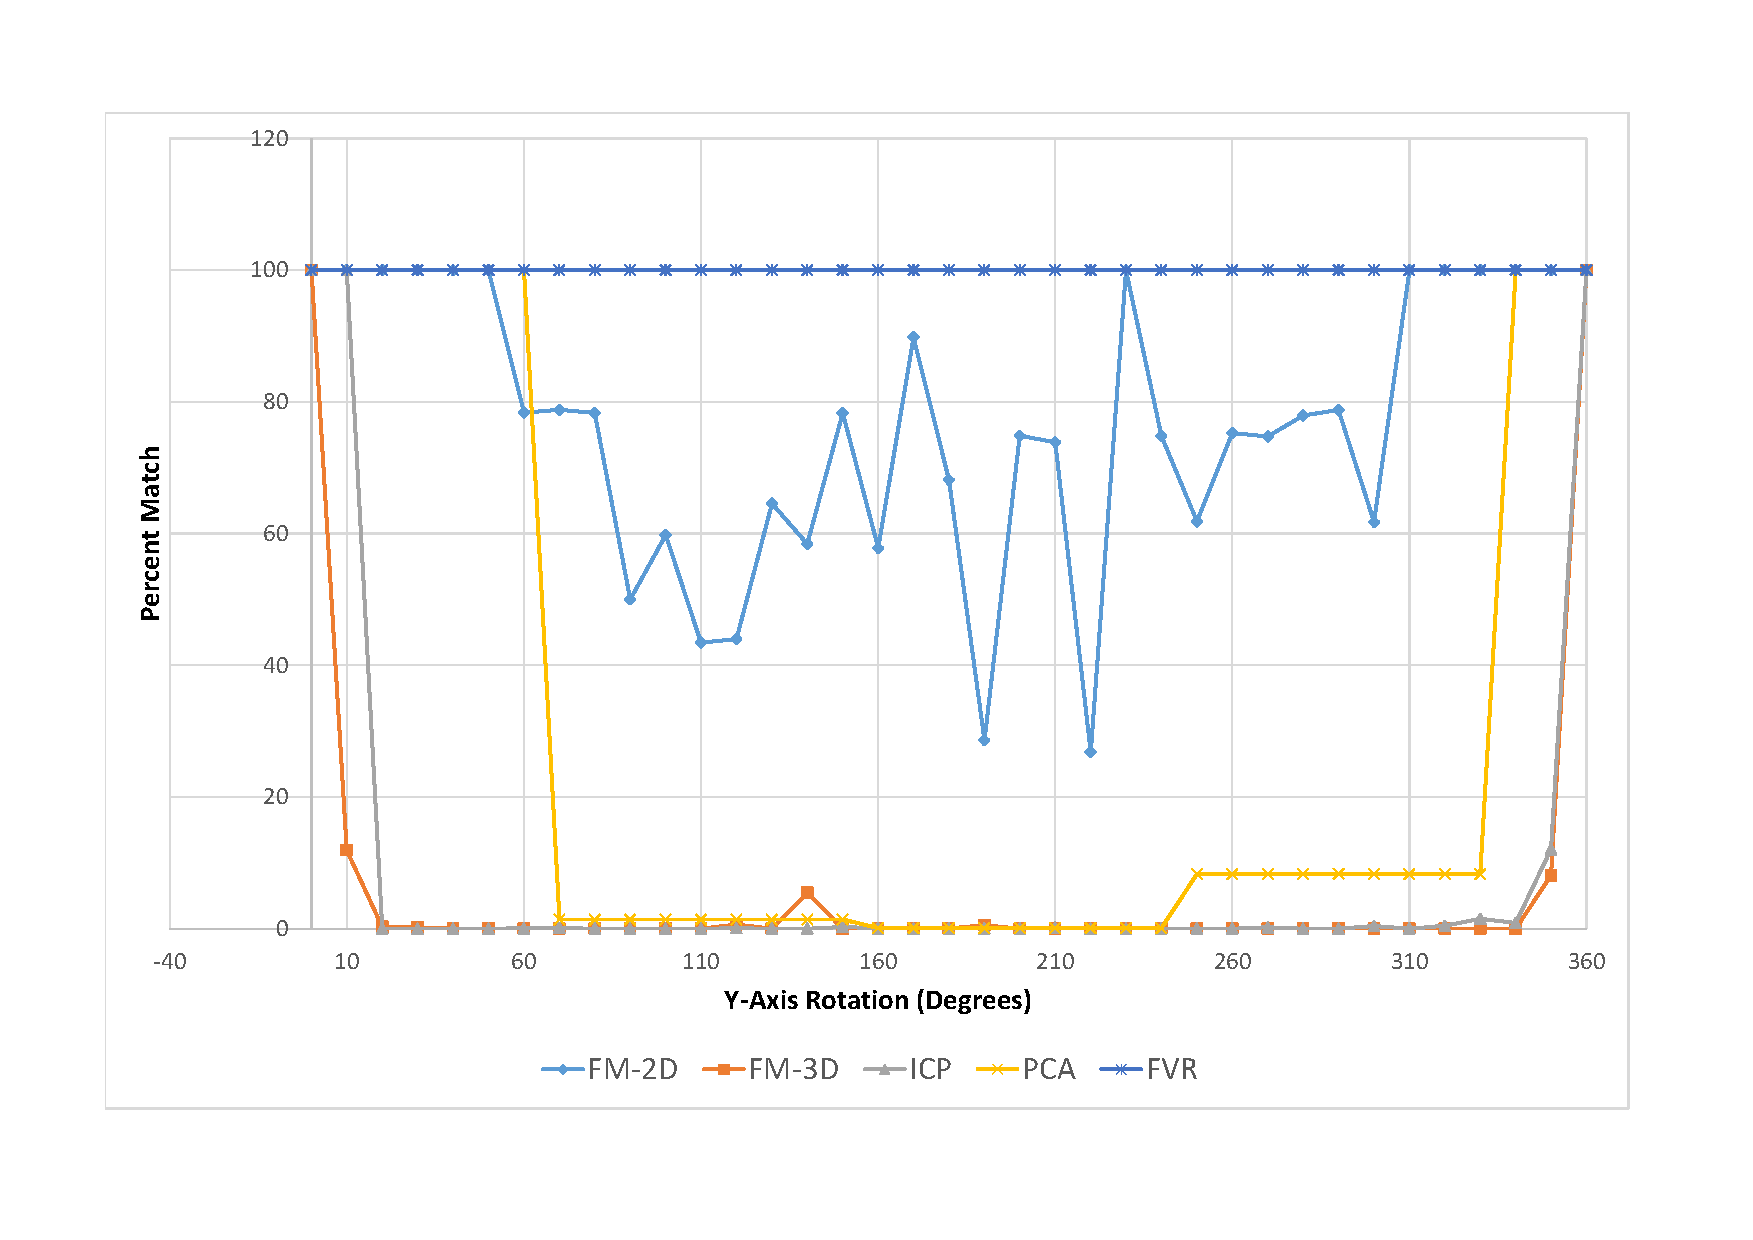
\includegraphics[width=4.0in]{images/results/noise/YRNoise2}
\caption{Percent Match for Y-Axis Registration with an SNR of 2580 and noise range of $2.0$.}
\label{fig:YRNoise2}
\end{figure}

In figure \ref{fig:YRNoise2} the SNR was reduced from $10300$ to $2580$. Again the 3D frame was rotated about the Y-axis prior to noise being added. The results were similar for ICP, FM-3D and PCA. These methods performed poorly with this amount of noise as well. The performance of the FM-2D method also appeared to steadily decline as the signal to noise ratio was lowered (noise was added). Again however, the FVR method had perfect registration accuracy for the estimation of this transform with this low a signal to noise ratio. \\

\subsubsection{Translation Registration}

The effects of noise on translation were also tested in these experiments. In the first experiment, 3D frames were translated by varying levels of x-axis translation. In the first experiment, different 3D reconstruction techniques were are compared using the percent match metric, to register translation transforms from 0 to 140 (in a frame space of $256^3$). Results are shown in figure \ref{figTNoise0}. In this figure, the 2D-FM, 3D-FM, PCA and FVR methods were shown to have perfect accuracy. This is expected as there is zero noise added prior to the registration of these 3D frames. ICP can be seen falling in terms of accuracy in translations with too wide a base-line (larger than 10 degrees). In this case, a possible solution may be to introduce scale space registration to ICP at an increase in complexity. \\  

\begin{figure}[!htb]
\centering
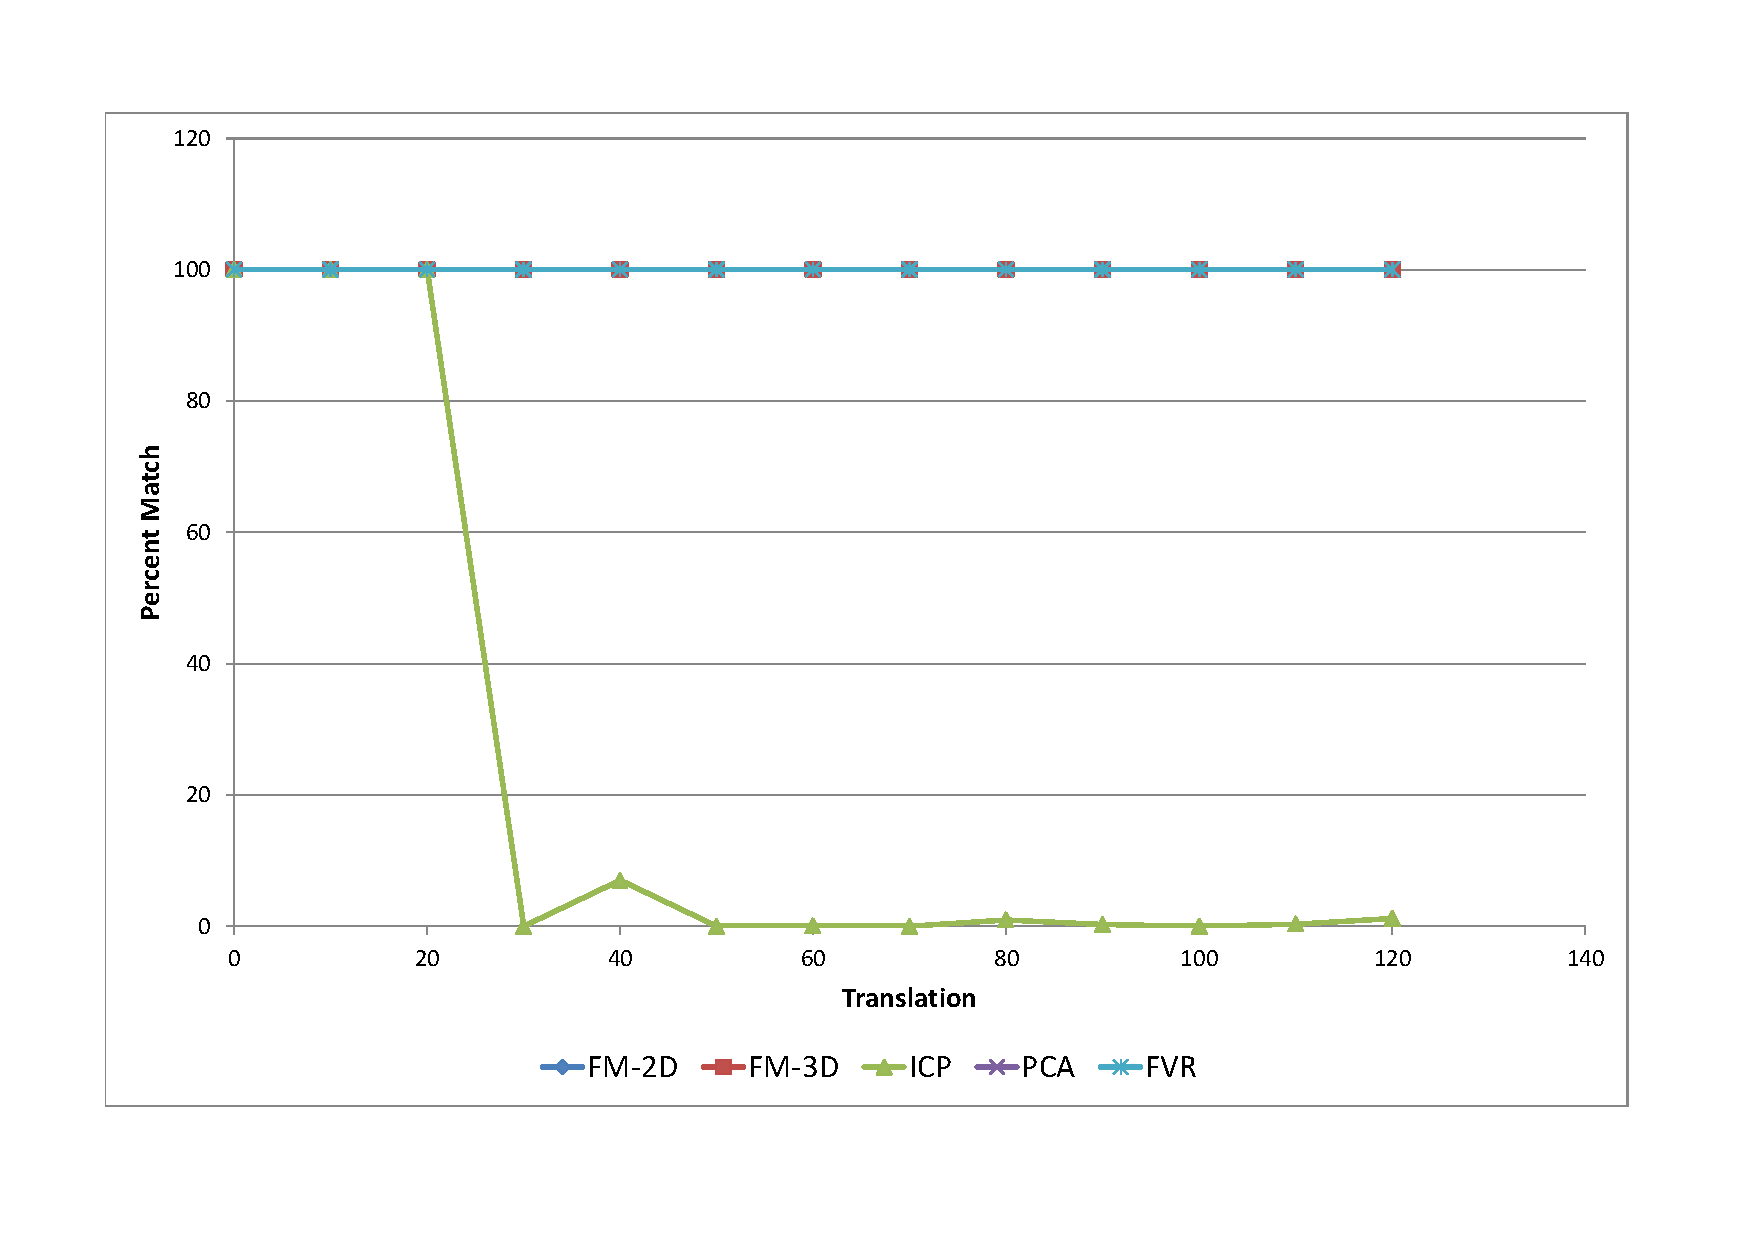
\includegraphics[width=4.0in]{images/results/noise/TransNoise0}
\caption{Percent Match for Translation Registration with an infinite SNR and noise range of $0$.}
\label{fig:TNoise0}
\end{figure}

Figure \ref{fig:TNoise1} shows the same experiment (documenting the effects of translation registration in the face of noise) with an increase in the level of noise added. Here, the SNR was decreased to $10300$ by adding noise prior to registration by each algorithm. With the exception of ICP, each algorithm seems to be equally robust at registering again translation at different levels of noise. Again, ICP is shown to be unable to handle wider baselines. In similar experiments where the signal to noise ratio was dropped further (figured \ref{fig:TNoise1} and \ref{fig:TNoise2}) similar results were found. \\


\begin{figure}[!htb]
\centering
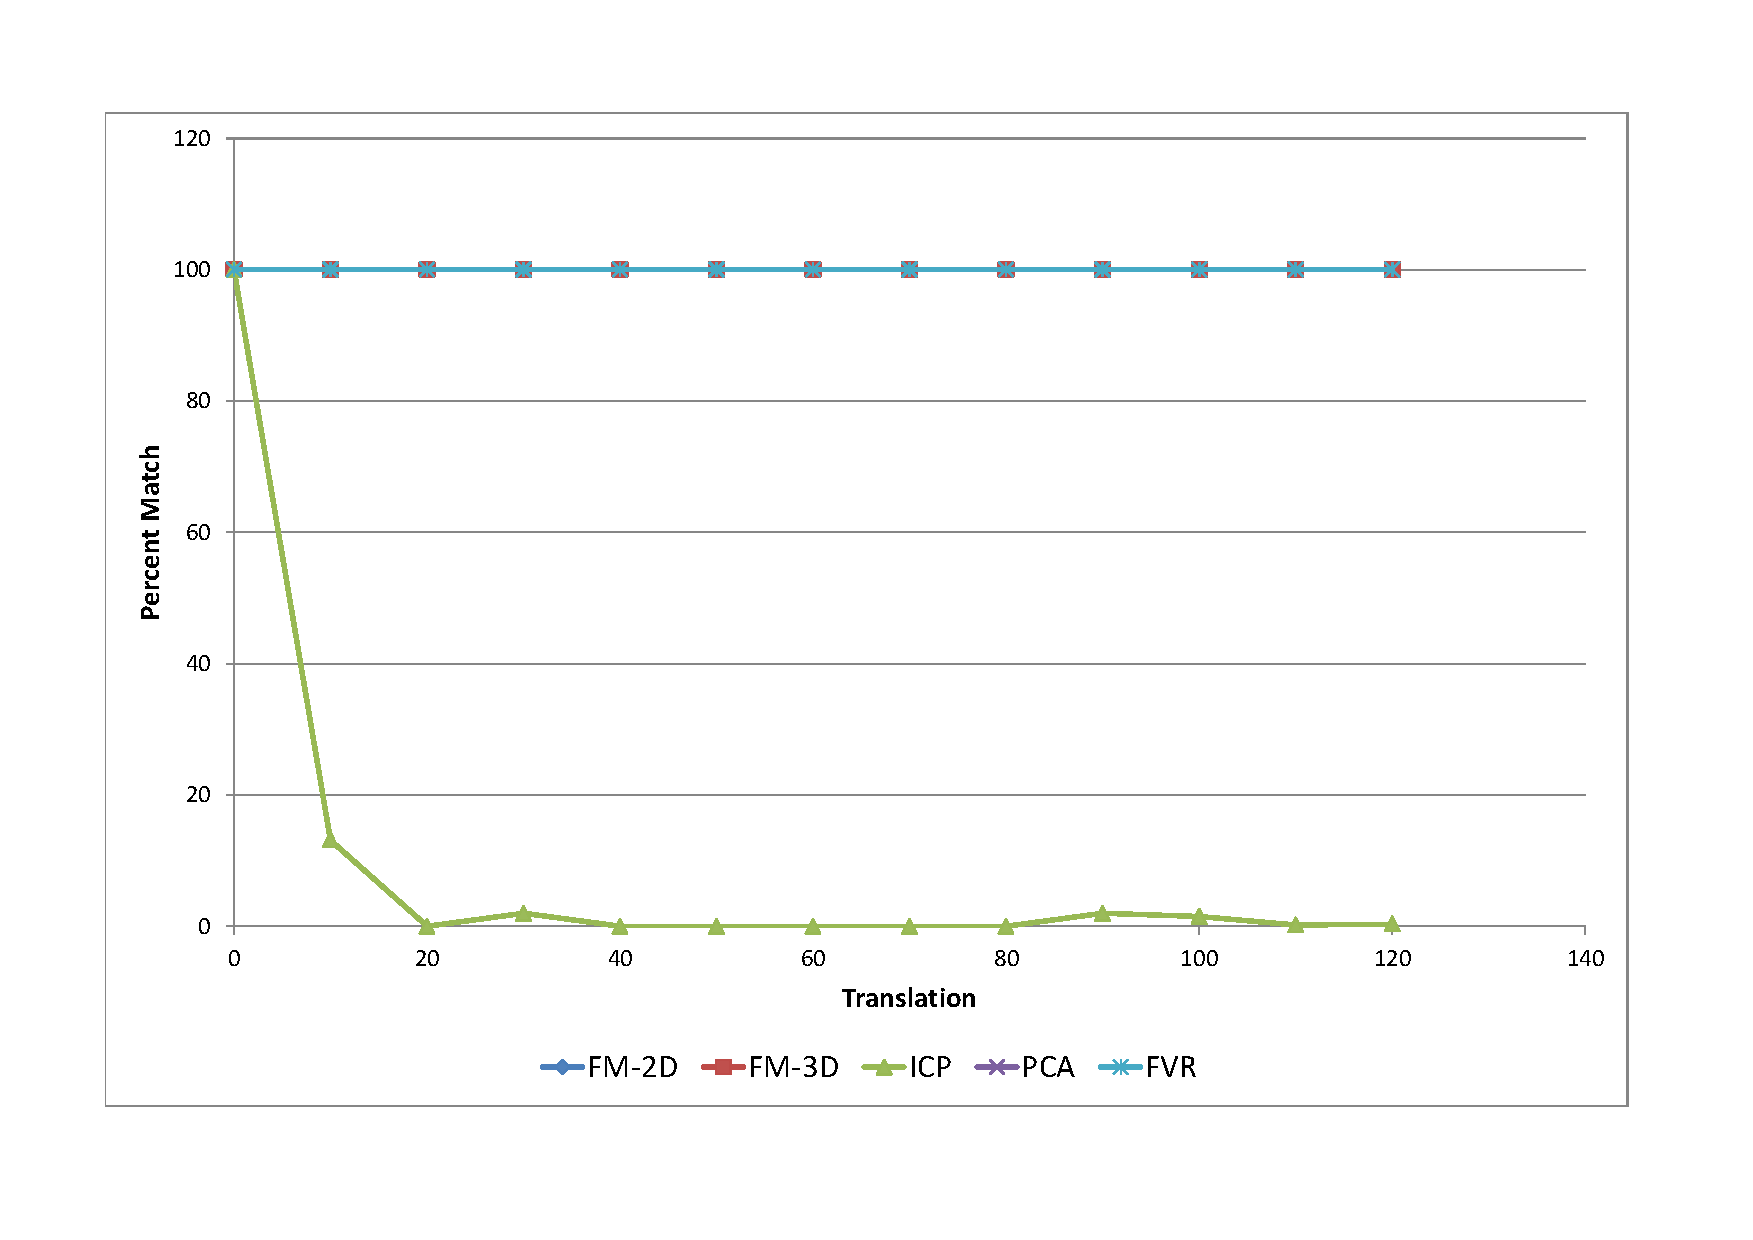
\includegraphics[width=4.0in]{images/results/noise/TransNoise1}
\caption{Percent Match for Translation Registration with an SNR of and noise range of $10300$ and noise range of $1.0$.}
\label{fig:TNoise1}
\end{figure}


\begin{figure}[!htb]
\centering
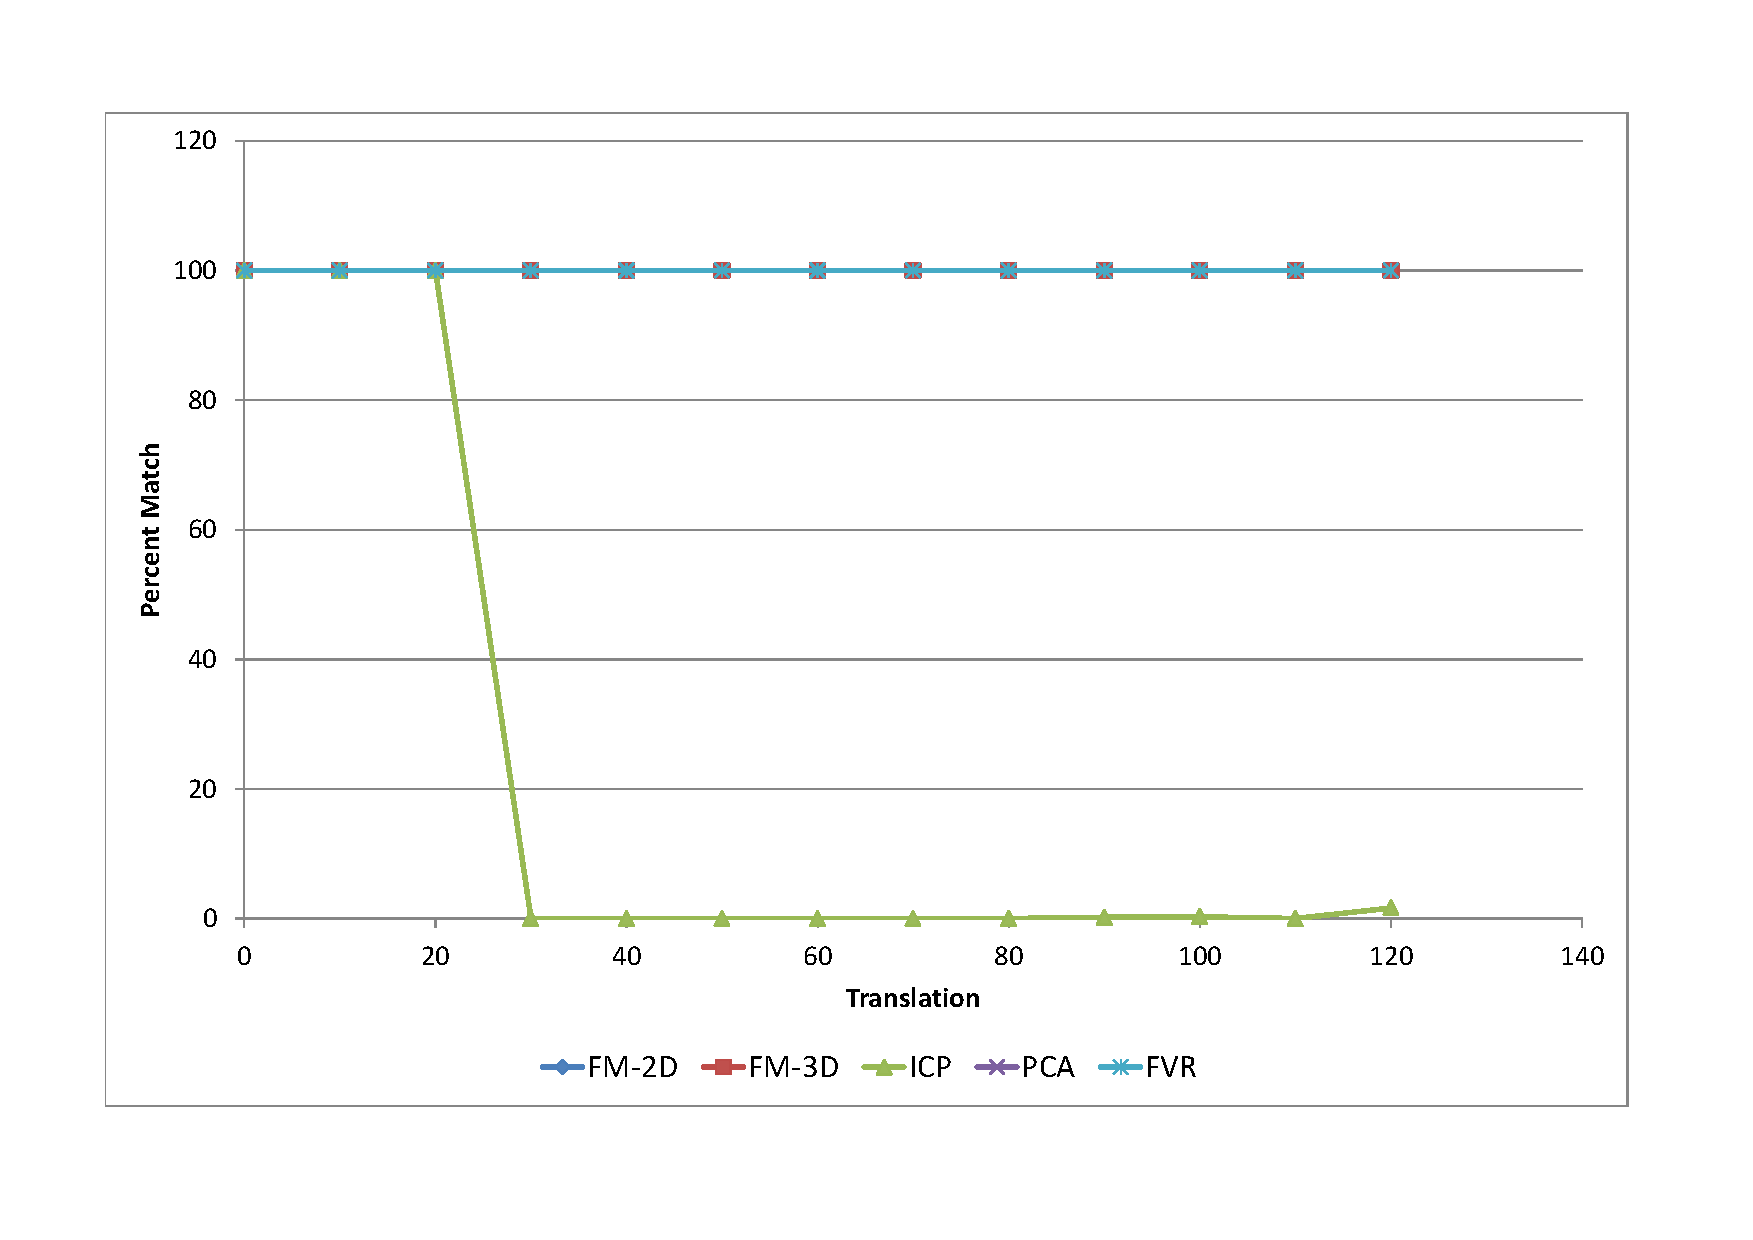
\includegraphics[width=4.0in]{images/results/noise/TransNoise2}
\caption{Percent Match for Translation Registration with an SNR of and noise range of $2580$ and noise range of $2.0$.}
\label{fig:TNoise2}
\end{figure}